\hypertarget{turtle__rect_8cpp}{}\section{tsim/src/turtle\+\_\+rect.cpp File Reference}
\label{turtle__rect_8cpp}\index{tsim/src/turtle\+\_\+rect.\+cpp@{tsim/src/turtle\+\_\+rect.\+cpp}}


Class Constructor for Turtle\+Rect.  


{\ttfamily \#include \char`\"{}tsim/turtle\+\_\+rect.\+h\char`\"{}}\newline
Include dependency graph for turtle\+\_\+rect.\+cpp\+:\nopagebreak
\begin{figure}[H]
\begin{center}
\leavevmode
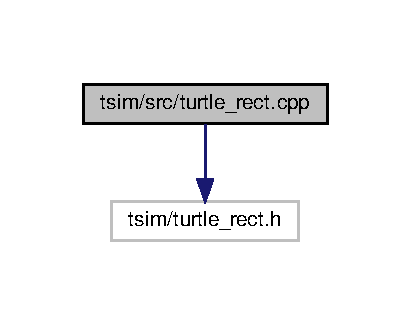
\includegraphics[width=197pt]{d7/df1/turtle__rect_8cpp__incl}
\end{center}
\end{figure}


\subsection{Detailed Description}
Class Constructor for Turtle\+Rect. 

P\+A\+R\+A\+M\+E\+T\+E\+RS\+: x\+\_\+ (int)\+: x coordinate for lower left corner of rectangle. y\+\_\+ (int)\+: y coordinate for lower left corner of rectangle. width\+\_\+ (int)\+: width of rectangle. height\+\_\+ (int)\+: height of rectangle. trans\+\_\+vel\+\_\+ (int)\+: translational velocity of robot. rot\+\_\+vel\+\_\+ (int)\+: rotational velocity of robot. frequency\+\_\+ (int)\+: frequency of control loop. threshold\+\_\+ (float)\+: specifies when the target pose has been reached.

goal\+\_\+x (float)\+: target turtle position in x. goal\+\_\+y (float)\+: target turtle position in y. goal\+\_\+head (float)\+: target turtle position in theta.

x\+\_\+pos\+\_\+ (float)\+: turtle position in x read from turtle1/pose topic. y\+\_\+pos\+\_\+ (float)\+: turtle position in y read from turtle1/pose topic. head\+\_\+ (float)\+: turtle position in theta read from turtle1/pose topic.

x\+\_\+o\+\_\+ (float)\+: turtle position in x predicted using forward model propagation. y\+\_\+o\+\_\+ (float)\+: turtle position in y predicted using forward model propagation. head\+\_\+o\+\_\+ (float)\+: turtle position in theta predicted using forward model propagation.

x\+\_\+error\+\_\+ (float)\+: turtle position error in x between read and predicted values. y\+\_\+error\+\_\+ (float)\+: turtle position error in y between read and predicted values. theta\+\_\+error\+\_\+ (float)\+: turtle position error in theta between read and predicted values.

pose\+\_\+error\+\_\+ (Pose\+Error)\+: custom message that stores x\+\_\+error, y\+\_\+error and theta\+\_\+error. twist\+\_\+ (Twist)\+: used to publish linear and angular velocities to turtle1/cmd\+\_\+vel.

done\+\_\+flag\+\_\+ (bool)\+: true when correct position or heading has been achieved in loop. lin\+\_\+ang\+\_\+flag\+\_\+ (bool)\+: true when angular velocity should be applied, linear otherwise. count)vertex\+\_\+ (int)\+: counter which resets to zero once all rectangle vertices have been reached.

F\+U\+N\+C\+T\+I\+O\+NS\+: traj\+\_\+reset\+Callback (bool)\+: callback for traj\+\_\+reset service, which teleports turtle back to initial config. pose\+Callback (void)\+: callback for turtle1/pose subscriber, which records the turtle\textquotesingle{}s pose for use elsewhere. move (void)\+: helper function which publishes Twist messages to turtle1/cmd\+\_\+vel to actuate the turtle. predict(void)\+: helper function which forward propagates the open-\/loop model and publishes Pose\+Error to pose\+\_\+error. control(void)\+: main class method. Houses state machine and calls helper function to perform trajectory and plot.

taken from \href{https://magiccvs.byu.edu/wiki/#!ros_tutorials/c++_node_class.md}{\tt https\+://magiccvs.\+byu.\+edu/wiki/\#!ros\+\_\+tutorials/c++\+\_\+node\+\_\+class.\+md} 